\section{引張弾塑性プレート}
この例では、中央に穴の開いた長方形のプレートに張力をかけています。
プレートは弾塑性材料でできています。対称性のため、プレートの1/4のみを解析します。\\
その寸法は:
\begin{itemize}
\item プレートサイズ:300$\times$150mm
\item 穴の直径:60 mm
\item 厚さ:10 mm
\end{itemize}
\begin{enumerate}
\item
  {[}mm, ton, s, °C{]}単位の新規ファイルを作成し、ステップ形式のジオメトリをPrePoMaxにインポートします。
  次に、パーツをメッシュ分割します。
  ここでは、最大要素サイズとして4mmを選択し、その他の設定は変更しませんでした(図\ref{fig:07-01})。
	\begin{figure}[H]
	\centering
	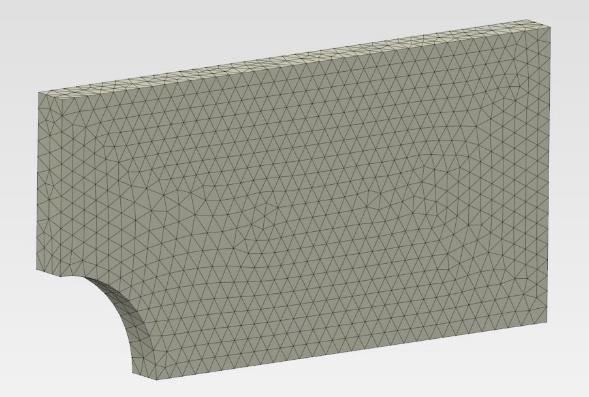
\includegraphics[width=83mm]{fig/07-01.png}
	\caption{プレート - メッシュ}
	\label{fig:07-01}
	\end{figure}
	\vspace{-\baselineskip}
\item
  新しい材料を定義し、弾性挙動を加え、ヤング率を210000MPa、ポアソン比を0.3と指定します。
  また、Plasticity(塑性)を追加し、以下のデータポイントを指定する(表\ref{tab:07-01})。
	\begin{table}[H]
	\centering
	\caption{プレート - 塑性定義のデータポイント}
	\label{tab:07-01}
	\begin{tabular}{|c|c|}
	\hline
	降伏応力 {[}MPa{]} & 塑性ひずみ{[}-{]} \\ \hline
	235 & 0  \\ \hline
	335 & 0.12  \\ \hline
	\end{tabular}
	\end{table}
	\vspace{-\baselineskip}
  先に作成した材料を参照して新しいソリッドセクションを作成し、そのセクションがこのパーツに割り当てられるように梁を選択します。
\item
  デフォルトの設定で静的ステップを定義します。
  対称性のためにカットされた面に変位/回転境界条件を適用します。
  それぞれのBCには、特定の面に垂直な方向に対応する自由度を固定します。
  変位/回転境界条件をもう1つ作成し、もっとも大きい2つの面に適用し、面外変形を防ぐために法線方向の変位を拘束します(実際には問題は2次元です)。
  プレートが引っ張られる側に-200MPaの圧力荷重をかけます(図\ref{fig:07-02})。
	\begin{figure}[H]
	\centering
	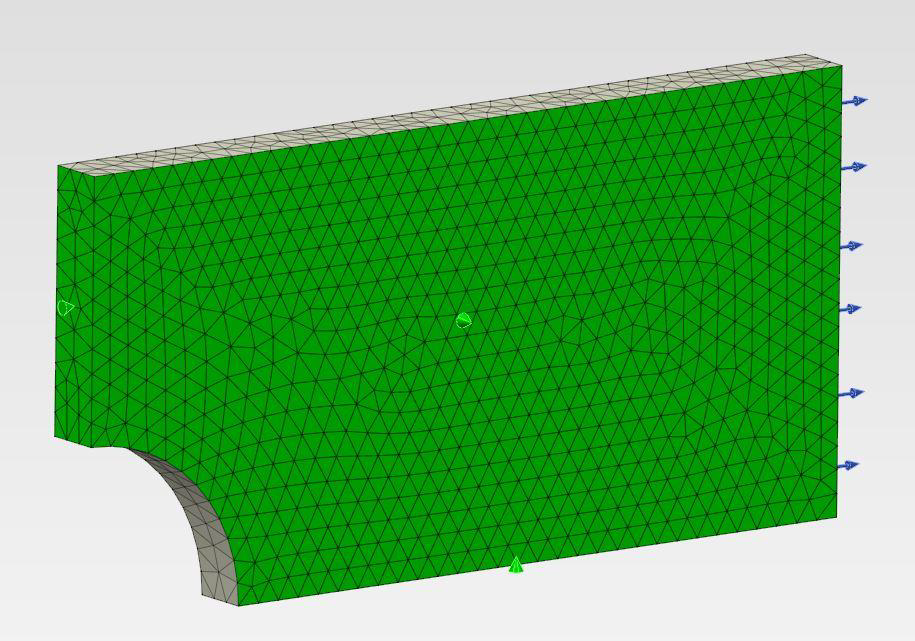
\includegraphics[width=105mm]{fig/07-02.png}
	\caption{プレート - 境界条件}
	\label{fig:07-02}
	\end{figure}
	\vspace{-\baselineskip}
\item
  新しいフィールド出力要求を追加し、要素出力とPEEQ変数を選択します。
\item
  解析を実行し、解析が完了したら結果を確認します。ミーゼス応力と塑性ひずみ(PE)の分布を詳しく見てみましょう(図\ref{fig:07-03})。
	\begin{figure}[H]
	\centering
	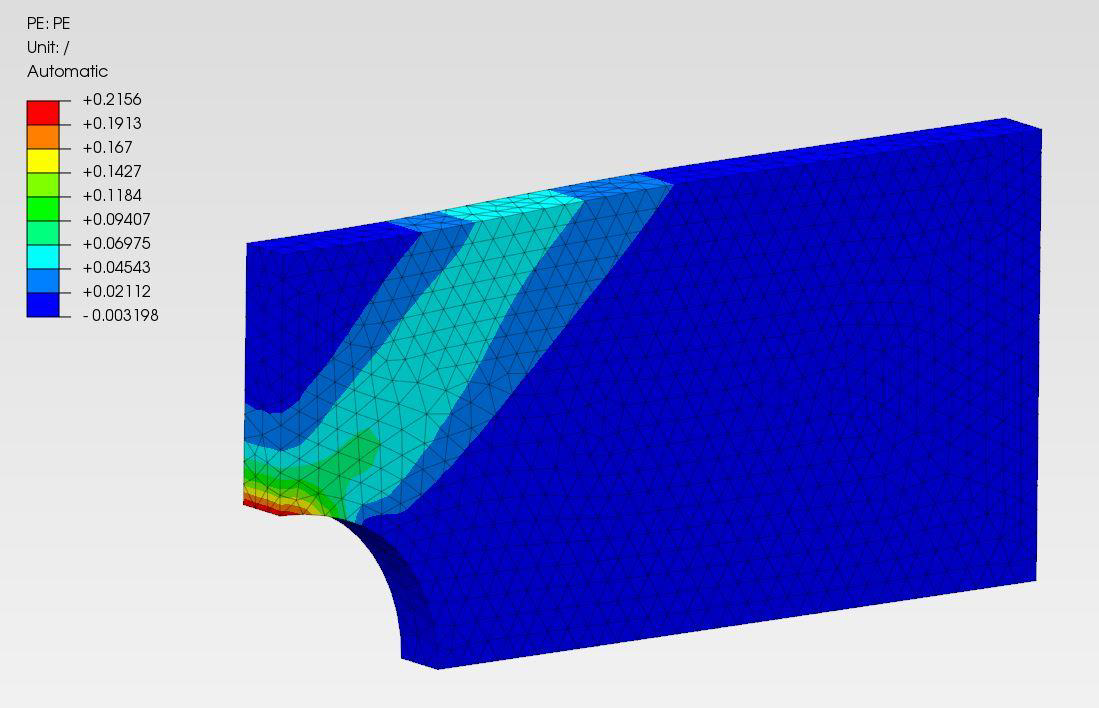
\includegraphics[width=115mm]{fig/07-03.png}
	\caption{プレート - 塑性ひずみ}
	\label{fig:07-03}
	\end{figure}
	\vspace{-\baselineskip}
\item
  Transformation → Symmetryオプションを使用して結果をミラーリングし、プレート全体の結果を表示します(図\ref{fig:07-04})。
	\begin{figure}[H]
	\centering
	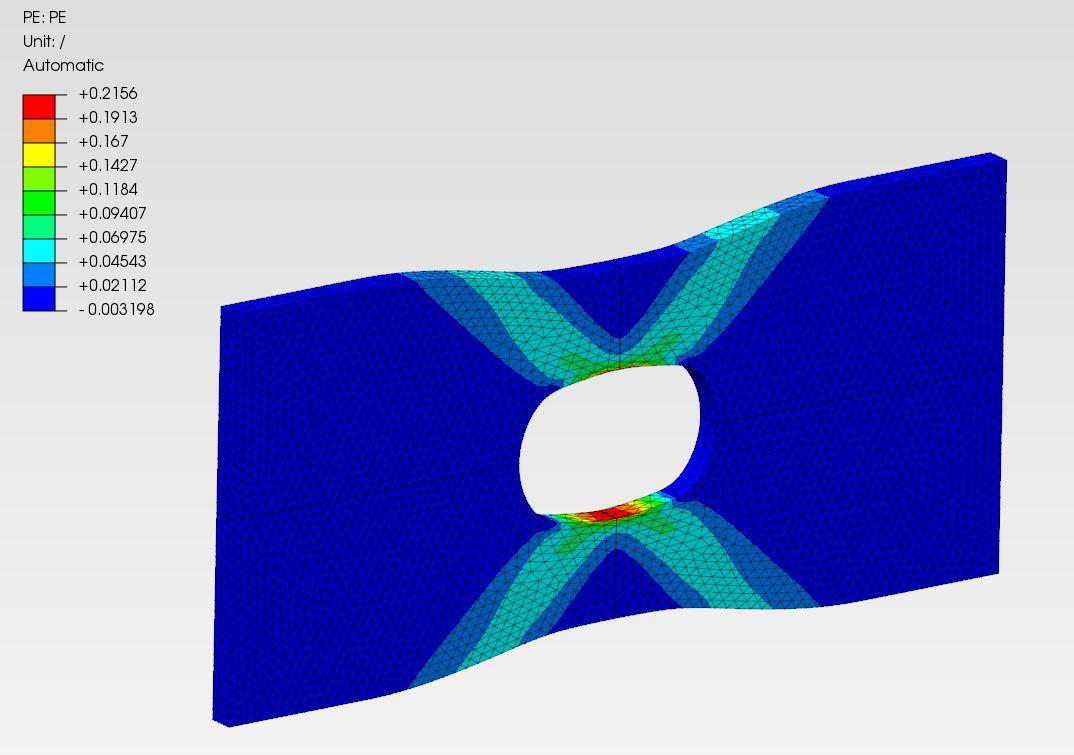
\includegraphics[width=132mm]{fig/07-04.png}
	\caption{プレート - 塑性ひずみ(ミラーリング)}
	\label{fig:07-04}
	\end{figure}
\end{enumerate}